% !TeX program = pdflatex
\documentclass[tikz,border=8pt]{standalone}
\usepackage{pgfplots}
\pgfplotsset{compat=1.16}
\definecolor{FigureBlue}{HTML}{2563EB}
\definecolor{FigureGreen}{HTML}{16A34A}
\definecolor{FigureOrange}{HTML}{EA580C}
\begin{document}
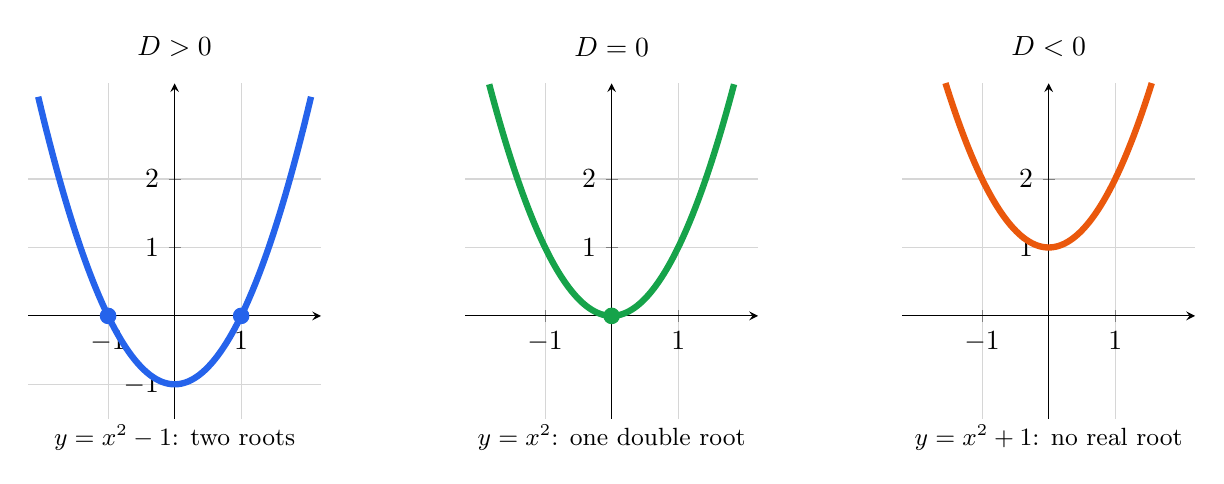
\begin{tikzpicture}
  \begin{axis}[
    width=5.3cm,height=6.1cm,axis lines=middle,xmin=-2.2,xmax=2.2,ymin=-1.8,ymax=3.4,
    title={$D>0$},xtick={-1,0,1},ytick={-1,0,1,2},grid=both,
    grid style={draw=gray!18},major grid style={draw=gray!32},clip=false,
  ]
    \addplot[FigureBlue,line width=2.3pt,domain=-2.05:2.05,samples=161] {x^2-1};
    \addplot[only marks,mark=*,mark size=2.8pt,FigureBlue] coordinates {(-1,0) (1,0)};
    \node[anchor=north,fill=white,inner sep=2pt,font=\small] at (axis cs:0,-1.5) {$y=x^2-1$: two roots};
  \end{axis}
  \begin{axis}[
    at={(5.55cm,0)},anchor=south west,width=5.3cm,height=6.1cm,axis lines=middle,
    xmin=-2.2,xmax=2.2,ymin=-1.8,ymax=3.4,title={$D=0$},xtick={-1,0,1},ytick={0,1,2},grid=both,
    grid style={draw=gray!18},major grid style={draw=gray!32},clip=false,
  ]
    \addplot[FigureGreen,line width=2.3pt,domain=-1.84:1.84,samples=161] {x^2};
    \addplot[only marks,mark=*,mark size=2.8pt,FigureGreen] coordinates {(0,0)};
    \node[anchor=north,fill=white,inner sep=2pt,font=\small] at (axis cs:0,-1.5) {$y=x^2$: one double root};
  \end{axis}
  \begin{axis}[
    at={(11.1cm,0)},anchor=south west,width=5.3cm,height=6.1cm,axis lines=middle,
    xmin=-2.2,xmax=2.2,ymin=-1.8,ymax=3.4,title={$D<0$},xtick={-1,0,1},ytick={0,1,2},grid=both,
    grid style={draw=gray!18},major grid style={draw=gray!32},clip=false,
  ]
    \addplot[FigureOrange,line width=2.3pt,domain=-1.55:1.55,samples=161] {x^2+1};
    \node[anchor=north,fill=white,inner sep=2pt,font=\small] at (axis cs:0,-1.5) {$y=x^2+1$: no real root};
  \end{axis}
\end{tikzpicture}
\end{document}
